\section{Im Programm verwendete und berechnete Werte}
Neben den Naturkonstanten
\begin{itemize}
    \item Masse des Elektrons $m$ =  $9,109 \cdot 10^{-31}$ in kg
    \item Ladung des Elektrons $e$ = $1,602 \cdot 10^{-19}$ in As
\end{itemize} 
benutzt das Programm verschiedene weitere Konstanten und Einstellungsparameter. 
Diese wurden zum Teil aus \cite{Gente1950} übernommen und zum Teil durch ausprobieren mit dem Programm ermittelt, sodass die Darstellung sinnvoll wird (zum Beispiel der Strahl nicht außerhalb der Röhre landet).
Im Einzelnen sind dies:
%\section{Konstanten}
\begin{itemize}
    \item Felddurchmesser $d$ = 30 in mm
    \item Bildschirmabstand $l$ = 500 in mm
    \item Beschleunigungsspannung $U_B$ im Bereich von $12 kV$ bis $16 kV$ und  zugehöriger Richtungsvektor $\vv{s} = \vektor{1}{0}{0}$ der Beschleunigungsstrecke.
    \item Magnetfeldstärke zweier Ablenkspulen:
    \begin{itemize}
        \item $B_1$ im Bereich $-5 mT$ bis $5 mT$, zugehöriger Richtungsvektor $\vv{b_1} = \vektor{0}{0}{1}$ % senkrechte Spule
        \item $B_2$ im Bereich $-5 mT$ bis $5 mT$, zugehöriger Richtungsvektor $\vv{b_2} = \vektor{0}{-1}{0}$ % waagerechte Spule
    \end{itemize}
\end{itemize}

In Abbildung \ref{fig:meineSimulation} ist zu sehen, wie die Einstellungsparameter geändert werden können. 
Des Weiteren werden die Werte für die zu berechnenden Werte ausgegeben:
%\section{Zu berechnende Parameter}
\begin{itemize}
    \item die Energie aus dem Ansatz (\ref{eq:Energie})
    \item Teilchengeschwindigkeit $v$ in $\frac{km}{s}$
    \item die Kräfte $F_1$ und $F_2$ aus dem Ansatz (\ref{eq:Kraft}) für senkrechtes und waagerechtes Spulenpaar
    %\item Ergebnisvektor $\vv{v}$
    \item Bahnradien $r_1$ und $r_2$ in mm 
    \item Ablenkwinkel $\alpha_1$ und $\alpha_2$ in Grad (Winkel werden auch in den Kreisen sichtbar)
    %\item Ablenkungsrichtung $\vv{a}$
\end{itemize}
Der am Ende von Abschnitt \ref{sec:g} berechnete Punkt $E$ ist im Bild als Endpunkt des blauen Strahls zu erkennen.
%\section{Programm und dessen steuerung}

\begin{figure}[h]
    \centering
    \includegraphics[width=1.2\textwidth]{fig/Fernseherröhre.PNG}
    \caption{Darstellung der Simulation}
    \label{fig:meineSimulation}
\end{figure}
%\paragraph{Einstellungsparameter:}

\pagebreak
\section{Graphische Ausarbeitung}
Wann immer man ein Objekt (Fernseheröhre oder jedes andere mögliche Objekt) auf einen Bildschirm abbilden möchte, muss man aus 3D in der "`Realität"' 2D auf dem Bildschirm machen. Dafür muss man eine Koordinatentransformation machen, welche auch als Kameratransformation bekannt ist \cite{Kameratransformation}.

\underline{$\vv{a}$ = Blickrichtung}
$$x = \sqrt{\frac{1}{6}}$$
$$y = \sqrt{\frac{2}{3}}$$
$$z = -\sqrt{\frac{1}{6}}$$
$$\vv{a}=\vektor{\sqrt{\frac{1}{6}}}{\sqrt{\frac{2}{3}}}{-\sqrt{\frac{1}{6}}} $$
$x$, $y$ sollen positiv sein, $z$ soll negativ sein und der Betrag/Länge soll 1 sein. $X$ etwas kleiner als $y$.
$$y= \sqrt{\frac{2}{3}}$$
$$x= \sqrt{\frac{1}{6}}$$
\underline{$\vv{b}$:}
$z$ = 0 ; andere Werte so wählen, dass Skalarprodukt 0 ergibt
$$x= \sqrt{\frac{2}{3}}$$
$$y=-\sqrt{\frac{1}{6}}$$
$$z=0$$
$$|\vv{b}| = \sqrt{\frac{5}{6}}\neq 1\mbox{ ; also müssen $x$ und $y$ mit dem Kehrwert von $\sqrt{\frac{5}{6}}$, also mit $\sqrt{\frac{6}{5}}$ multipliziert werden.}$$
$$x' = \sqrt{\frac{12}{15}} = \sqrt{\frac{4}{5}}$$
$$y' = - \sqrt{\frac{1}{5}}$$
$$z' = 0$$
$$\vv{b}= \vektor{\sqrt{\frac{4}{5}}}{-\sqrt{\frac{1}{5}}}{0}$$
\underline{$\vv{c}$:}
$$\vv{c} = \vv{b}\times  \vv{a}$$
$$= \vektor{\frac{4}{5}}{-\sqrt{\frac{1}{5}}}{0}
      \times \vektor{\sqrt{\frac{1}{6}}}{\sqrt{\frac{2}{3}}}{-\sqrt{\frac{1}{6}}} \mbox{ = } 
     \left(\begin{array}{c} 
     \frac{\sqrt{5}}{5}\cdot\frac{\sqrt{6}}{6}\\2\cdot\frac{\sqrt{5}}{5}\cdot\frac{\sqrt{6}}{6}\\2\cdot\frac{\sqrt{5}}{5}\cdot\frac{\sqrt{6}}{3}+\frac{\sqrt{5}}{5}\cdot\frac{\sqrt{6}}{6}\end{array}\right)
$$
Wir suchen eine Matrix $A$, sodass

     $$A\cdot \vv{a}=\vektor{0}{1}{0}\mbox{ ist ;} $$
     $$A\cdot \vv{b}=\vektor{1}{0}{0}\mbox{ ist ;}$$
     $$A\cdot \vv{c}=\vektor{0}{0}{1}\mbox{ ist ;} $$
     
$$\mbox{$B$ = } \m{\sqrt{\frac{4}{5}}}{\sqrt{\frac{1}{6}}}{\frac{\sqrt{5}}{5} \cdot \frac{\sqrt{6}}{6}}{-\sqrt{\frac{1}{5}}}{\sqrt{\frac{2}{3}}}{2 \cdot \frac{\sqrt{5}}{5} \cdot \frac{\sqrt{6}}{6}}{0}{-\sqrt{\frac{1}{6}}}{2 \cdot \frac{\sqrt{5}}{5} \cdot \frac{\sqrt{6}}{3} + \frac{\sqrt{5}}{5} \cdot \frac{\sqrt{6}}{6}}$$
Um auf die Matrix $A$ zu kommen, muss man nun die Matrix $B$ mit Hilfe von GeoGebra invertieren:
$$\mbox{$A$ = } \m {2\cdot\frac{\sqrt{5}}{5}}{-\frac{\sqrt{5}}{5}}{0}{\frac{\sqrt{6}}{6}}{\frac{\sqrt{6}}{3}}{-\frac{\sqrt{6}}{6}}{\frac{\sqrt{30}}{30}}{\frac{\sqrt{30}}{15}}{\frac{\sqrt{30}}{6}}$$
Wir verwenden $A$, um aus einem $(x,y,z)$ Vektor $\vv{v}$ ein zweidimensionales Koordinatenpaar zu kriegen, indem wir $ A \cdot \vv{v} = \m {2\cdot\frac{\sqrt{5}}{5}}{-\frac{\sqrt{5}}{5}}{0}{\frac{\sqrt{6}}{6}}{\frac{\sqrt{6}}{3}}{-\frac{\sqrt{6}}{6}}{\frac{\sqrt{30}}{30}}{\frac{\sqrt{30}}{15}}{\frac{\sqrt{30}}{6}} \cdot \vektor{v.x}{v.y}{v.z}$ rechnen um den Vektor $ \vektor{x_1}{-}{y_1}$ rauszubekommen, wobei die $y$-Koordinate ignorieren.  
%\section{Simulation}
%\subsection{a}
%\subsection{b}
\section{zusätzliche Abbildungen}

\begin{figure}[h]
    \centering
    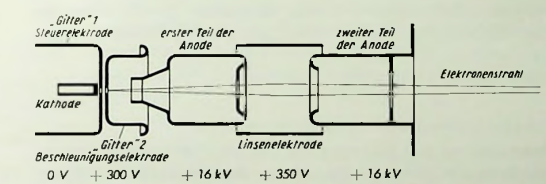
\includegraphics[width=.9\textwidth]{fig/Elektronenstrahl.PNG}
    \caption{Darstellung der Elektronenkanone (übernommen aus dem Buch \cite{Fernsehroehre})}
    \label{fig:elS}
\end{figure}

\begin{figure}[h]
    \centering
    \includegraphics[width=.75\textwidth]{fig/Fernsehröhre.jpg}
    \caption{Abbildung des Inneren der Fernsehröhre (übernommen von \cite{Abbildung}) }
    \label{fig:Fernsehroehre}
\end{figure}
